\documentclass[a4paper,9pt]{extarticle}

% --- PACKAGES ESSENTIELS ---
\usepackage[utf8]{inputenc}
\usepackage[T1]{fontenc}
\usepackage{helvet}
\renewcommand{\familydefault}{\sfdefault}

\usepackage[left=0.8cm, right=0.8cm, top=0.55cm, bottom=0.55cm]{geometry}
\usepackage{xcolor}
\usepackage{titlesec}
\usepackage{enumitem}
\usepackage{tabularx}
\usepackage{fontawesome5}
\usepackage[hidelinks]{hyperref}
\usepackage{tikz}

\pagestyle{empty}

% --- COULEURS PROFESSIONNELLES & MODERNES (GÉNIE INDUSTRIEL & SUPPLY CHAIN) ---
\definecolor{primary}{HTML}{0F172A}      % Deep Slate / Bleu Nuit Industriel (#0F172A)
\definecolor{accent}{HTML}{1D4ED8}       % Bleu Royal Cobalt (#1D4ED8)
\definecolor{accentteal}{HTML}{0D9488}   % Sarcelle Émeraude / Lean & Green Supply Chain (#0D9488)
\definecolor{textdark}{HTML}{1E293B}     % Texte principal très lisible
\definecolor{textmuted}{HTML}{475569}    % Métadonnées / Dates / Lieux
\definecolor{linegray}{HTML}{CBD5E1}     % Séparateurs discrets
\definecolor{tagbg}{HTML}{F8FAFC}        % Arrière-plan badges
\definecolor{tagborder}{HTML}{CBD5E1}    % Bordure badges

% --- CONFIGURATION DES LIENS ---
\hypersetup{
    colorlinks=true,
    urlcolor=accent,
    linkcolor=accent
}

% Supprimer les warnings hyperref pour les glyphes FontAwesome
\pdfstringdefDisableCommands{%
  \def\faUser{}%
  \def\faBriefcase{}%
  \def\faCogs{}%
  \def\faGraduationCap{}%
  \def\faCubes{}%
  \def\faAward{}%
  \def\faLanguage{}%
  \def\faHeart{}%
  \def\faExternalLink*{}%
  \def\faCalendar*{}%
  \def\faMapMarker*{}%
  \def\faPhone*{}%
  \def\faEnvelope{}%
  \def\faLinkedin{}%
  \def\faWrench{}%
  \def\faLightbulb{}%
}

% --- FORMAT DES TITRES DE SECTION ---
\titleformat{\section}
  {\color{primary}\bfseries\small}
  {}{0em}
  {}[\vspace{-2.5pt}{\color{accent}\rule{\linewidth}{1.1pt}}\vspace{-2.5pt}]

\titlespacing{\section}{0pt}{3pt}{1.5pt}

% --- LISTES COMPACTES ---
\setlist[itemize]{
  noitemsep,
  topsep=0.8pt,
  parsep=0pt,
  partopsep=0pt,
  leftmargin=8.5pt,
  label={\color{accent}\scriptsize\faAngleRight}
}

% --- MACROS PERSONNALISÉES ---
\newcommand{\cvhighlight}[1]{\textcolor{accentteal}{\textbf{#1}}}
\newcommand{\cvtech}[1]{\textcolor{primary}{\textbf{#1}}}

\newcommand{\cvtag}[1]{%
  \tikz[baseline=-0.5ex]\node[draw=tagborder, fill=tagbg, rounded corners=2pt, inner xsep=2.2pt, inner ysep=0.8pt, font=\fontsize{6pt}{7pt}\selectfont\sffamily\color{primary}]{#1};%
}

\setlength{\parindent}{0pt}
\setlength{\parskip}{0pt}

\begin{document}

%=============================================================================
% EN-TÊTE DU CV AVEC PHOTO (HEADER)
%=============================================================================
\noindent
\begin{tabularx}{\linewidth}{@{} X r @{}}
  \begin{minipage}[c]{0.82\linewidth}
    {\LARGE \textbf{\color{primary} HOUDA TAZI}}\\[2pt]
    {\small \textbf{\color{accent} ÉLÈVE-INGÉNIEURE D'ÉTAT EN 5\textsuperscript{ÈME} ANNÉE -- GÉNIE INDUSTRIEL}}\\[2pt]
    {\footnotesize \color{textmuted} À la recherche d'une opportunité en \textbf{\color{primary}Production, Amélioration Continue (Lean), Supply Chain \& Logistique} | 2026}\\[3pt]
    {\footnotesize \color{textdark}
      \faEnvelope\ \href{mailto:tazihouda1108@gmail.com}{tazihouda1108@gmail.com} \quad\textbar\quad
      \faPhone*\ \href{tel:+212695957464}{+212 695-957464} \quad\textbar\quad
      \faLinkedin\ \href{https://www.linkedin.com/in/houda-tazi-625b11389}{linkedin.com/in/houda-tazi} \quad\textbar\quad
      \faMapMarker*\ Berrechid / Casablanca
    }
  \end{minipage}
  &
  \begin{tikzpicture}[baseline=(current bounding box.center)]
    \clip (0,0) circle (1.12cm);
    \node at (0,0) {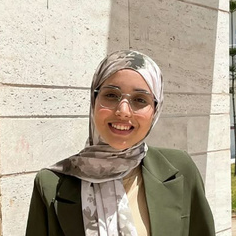
\includegraphics[width=2.3cm]{houda_photo.png}};
    \draw[line width=1.4pt, color=accent] (0,0) circle (1.12cm);
  \end{tikzpicture}
\end{tabularx}

\vspace{1pt}
\noindent{\color{linegray}\rule{\linewidth}{0.7pt}}
\vspace{1pt}

%=============================================================================
% CORPS DU CV : MISE EN PAGE 2 COLONNES (58.5% GAUCHE / 39.5% DROITE)
%=============================================================================
\noindent
\begin{minipage}[t]{0.585\textwidth}

  %----------- PROFIL -----------
  \section{\faUser\ Profil Professionnel}
  {\footnotesize \color{textdark}
  Élève-Ingénieure d'État en dernière année à l'\textbf{ENSA El Jadida}, spécialisée en \cvhighlight{Génie Industriel}. Forte d'expériences pratiques auprès de leaders de référence (\textbf{Leoni, SEWS Cabind, Groupe OCP}), je maîtrise l'optimisation des flux, le \cvtech{Lean Manufacturing (5S, Kaizen, VSM, SMED)}, le pilotage de la performance (\cvhighlight{TRS / OEE, MSP}) et la modélisation sous \cvtech{CPLEX / Arena}. Rigoureuse et orientée terrain, je souhaite mettre mes compétences au service de l'excellence opérationnelle.
  }

  \vspace{1.5pt}

  %----------- EXPÉRIENCES PROFESSIONNELLES -----------
  \section{\faBriefcase\ Expériences Professionnelles}

  % LEONI
  \textbf{\color{primary} Stagiaire Ingénieure -- Amélioration Continue (PFE)} \hfill {\scriptsize\color{textmuted}\faCalendar*\ 01/2026 -- 08/2026}\\
  {\footnotesize \textbf{\color{accent} LEONI WIRING SYSTEMS}} \hfill {\scriptsize\color{textmuted}\faMapMarker*\ Berrechid, Maroc}
  \begin{itemize}
    \item Sujet : \textit{Amélioration de l'efficience de la ligne LAD MERGE P2JO PPL (Câblage Auto)}.
    \item Cartographie des flux de valeur (\cvhighlight{VSM}) et détection des gaspillages (\cvhighlight{Muda}).
    \item Équilibrage des postes de travail par chrono-analyse et standardisation opératoire.
    \item Déploiement d'outils Lean (\cvtech{Kaizen, 5S, Standard Work, Poka-Yoke}) et gestion des encours.
    \item Suivi des indicateurs clés : Taux de Rendement Synthétique (\cvhighlight{TRS / OEE}) et cadence.
  \end{itemize}
  \vspace{1pt}
  {\scriptsize \textbf{\color{textmuted}Outils :}\ \cvtag{Lean Manufacturing} \cvtag{VSM} \cvtag{Chrono-analyse} \cvtag{TRS / OEE} \cvtag{5S / Kaizen}}

  \vspace{2pt}

  % SEWS CABIND
  \textbf{\color{primary} Stagiaire Ingénieure Génie Industriel (Application)} \hfill {\scriptsize\color{textmuted}\faCalendar*\ 06/2025 -- 09/2025}\\
  {\footnotesize \textbf{\color{accent} SEWS-CABIND MAROC (Sumitomo Electric)}} \hfill {\scriptsize\color{textmuted}\faMapMarker*\ Casablanca, Maroc}
  \begin{itemize}
    \item Sujet : \textit{Amélioration de la productivité LAD -- Projet PORTA DUCATO MY21}.
    \item Chronométrage, analyse des temps de cycle et réduction des micro-arrêts d'assemblage.
    \item Réorganisation ergonomique des postes et rééquilibrage de ligne pour absorber les pics.
    \item Déploiement du \cvhighlight{management visuel} et standardisation des gammes opératoires (\cvtech{SOP}).
  \end{itemize}
  \vspace{1pt}
  {\scriptsize \textbf{\color{textmuted}Outils :}\ \cvtag{Productivité} \cvtag{Équilibrage de Ligne} \cvtag{Management Visuel} \cvtag{Ergonomie}}

  \vspace{2pt}

  % OCP / PMP
  \textbf{\color{primary} Stagiaire Ingénieure Procédés \& Méthodes (Initiation)} \hfill {\scriptsize\color{textmuted}\faCalendar*\ 08/2024 -- 08/2024}\\
  {\footnotesize \textbf{\color{accent} PAKISTAN MAROC PHOSPHORE -- GROUPE OCP}} \hfill {\scriptsize\color{textmuted}\faMapMarker*\ Jorf Lasfar, Maroc}
  \begin{itemize}
    \item Sujet : \textit{Bilan matière (1800 T P2O5/j) en attaque-filtration et détection des goulots}.
    \item Bilan massique et analyse des pertes sur l'unité d'acide phosphorique.
    \item Détection des \cvhighlight{goulots d'étranglement} selon la Théorie des Contraintes (TOC).
    \item Recommandations techniques d'optimisation du rendement et de stabilité de filtration.
  \end{itemize}
  \vspace{1pt}
  {\scriptsize \textbf{\color{textmuted}Outils :}\ \cvtag{Bilan Matière} \cvtag{Théorie des Contraintes} \cvtag{Génie Chimique} \cvtag{OCP Group}}

  \vspace{1.5pt}

  %----------- PROJETS D'INGÉNIERIE -----------
  \section{\faCogs\ Projets d'Ingénierie \& d'Application}

  % ECOBITE
  \textbf{\color{primary} Projet ECOBITE -- IA \& Logistique Inverse Durable} \hfill {\scriptsize\color{textmuted}\faCalendar*\ 2025 -- 2026}\\
  {\scriptsize\color{textmuted} Revalorisation durable des déchets alimentaires en nutrition animale}
  \begin{itemize}
    \item Modélisation de la \cvhighlight{logistique inverse} (collecte, traçabilité et valorisation).
    \item Optimisation des tournées par IA pour minimiser coûts logistiques et empreinte carbone.
  \end{itemize}
  \vspace{1pt}
  {\scriptsize \textbf{\color{textmuted}Domaines :}\ \cvtag{Logistique Inverse} \cvtag{Supply Chain Verte} \cvtag{IA} \cvtag{Optimisation}}

  \vspace{2pt}

  % OPTIMISATION CONTENEURS
  \textbf{\color{primary} Optimisation Logistique du Chargement de Conteneurs (PFA 2)} \hfill {\scriptsize\color{textmuted}\faCalendar*\ 2024 -- 2025}\\
  {\scriptsize\color{textmuted} Résolution du Problème du Sac à Dos (Knapsack Problem) en transport fret}
  \begin{itemize}
    \item Modélisation en \cvhighlight{Programmation Linéaire (PLNE)} sous \cvtech{IBM ILOG CPLEX} et \cvtech{Python}.
    \item Maximisation du taux de remplissage volumétrique des conteneurs maritimes.
  \end{itemize}
  \vspace{1pt}
  {\scriptsize \textbf{\color{textmuted}Outils :}\ \cvtag{IBM ILOG CPLEX} \cvtag{Python} \cvtag{Recherche Opérationnelle}}

  \vspace{2pt}

  % ERP & PROTOTYPE CATIA
  \textbf{\color{primary} Prototype Manutention (CATIA V5) \& ERP Achats (VBA/MySQL)} \hfill {\scriptsize\color{textmuted}\faCalendar*\ 2024}\\
  \begin{itemize}
    \item Conception CAO 3D (\cvtech{CATIA V5}) d'un convoyeur étanche d'engrais portuaires.
    \item Développement ERP sous \cvtech{Excel VBA} avec BDD \cvtech{MySQL} (MCD/MLD) pour stocks et achats.
    \item Analyse des risques industriels par la méthodologie \cvhighlight{AMDEC Process} (Atlas Plastic's).
  \end{itemize}
  \vspace{1pt}
  {\scriptsize \textbf{\color{textmuted}Outils :}\ \cvtag{CATIA V5} \cvtag{Excel VBA} \cvtag{MySQL} \cvtag{AMDEC Process}}

\end{minipage}
\hfill
%=============================================================================
% COLONNE DE DROITE (SIDEBAR : 39.5% DE LARGEUR)
%=============================================================================
\begin{minipage}[t]{0.395\textwidth}

  %----------- FORMATION -----------
  \section{\faGraduationCap\ Formation}

  \textbf{\color{primary}\small Diplôme d'Ingénieur d'État} \hfill {\scriptsize\color{textmuted}\faCalendar*\ 2023 -- 2026}\\
  {\small \textbf{ENSA El Jadida}}\\
  {\footnotesize École Nationale des Sciences Appliquées}\\
  {\footnotesize Filière : \cvhighlight{Génie Industriel}}\\
  {\scriptsize\textit{5\textsuperscript{ème} année (Dernière année -- Promotion 2026)}}

  \vspace{1.5pt}

  \textbf{\color{primary}\small Classes Préparatoires Intégrées} \hfill {\scriptsize\color{textmuted}\faCalendar*\ 2021 -- 2023}\\
  {\small \textbf{ENSA El Jadida}}\\
  {\footnotesize Mathématiques, Physique \& Sciences de l'Ingénieur}

  \vspace{1.5pt}

  \textbf{\color{primary}\small Baccalauréat Sciences Physiques} \hfill {\scriptsize\color{textmuted}\faCalendar*\ 2020 -- 2021}\\
  {\small \textbf{Lycée Othmane Ben Affane, El Gara}}\\
  {\footnotesize Option Français}

  \vspace{2pt}

  %----------- COMPÉTENCES CLÉS -----------
  \section{\faCubes\ Compétences Clés}

  {\footnotesize \textbf{\color{accent} Lean Manufacturing \& Qualité}}
  \begin{itemize}
    \item 5S, Kaizen, SMED, VSM, Kanban, TPM
    \item TRS / OEE, Équilibrage de postes, Muda
    \item Maîtrise Statistique des Procédés (MSP / SPC)
    \item MiniTab, Six Sigma, AMDEC, 8D, Poka-Yoke
  \end{itemize}

  \vspace{1.5pt}
  {\footnotesize \textbf{\color{accent} Supply Chain \& Gestion Industrielle}}
  \begin{itemize}
    \item Planification de production (PIC, PDP, CBN)
    \item Gestion des stocks \& approvisionnements
    \item Logistique des flux \& logistique inverse
    \item ERP / GPAO : Odoo, Excel VBA, Systèmes d'Info
    \item Gestion des risques industriels \& HSE
  \end{itemize}

  \vspace{1.5pt}
  {\footnotesize \textbf{\color{accent} Modélisation \& Simulation}}
  \begin{itemize}
    \item IBM ILOG CPLEX (Optimisation PLNE)
    \item Arena (Simulation de flux de production)
    \item CATIA V5 (Conception mécanique 3D, Dessin)
    \item MATLAB, Simulink, Cartographie de flux
  \end{itemize}

  \vspace{1.5pt}
  {\footnotesize \textbf{\color{accent} Informatique \& Systèmes d'Info}}
  \begin{itemize}
    \item Python (Analyse de données, pandas, numpy)
    \item C/C++ (POO), MySQL, MCD/MLD
    \item Excel Avancé / VBA (Macros \& Dashboards)
    \item TIA Portal (Automatisme industriel), Web
  \end{itemize}

  \vspace{2pt}

  %----------- CONNAISSANCES TECHNIQUES -----------
  \section{\faWrench\ Connaissances Techniques}
  {\footnotesize
    \textbf{Électromécanique :} Machines électriques, thermiques (IMV, IMG), circuits et machines hydrauliques.
  }

  \vspace{2pt}

  %----------- SOFT SKILLS -----------
  \section{\faLightbulb\ Savoir-Être \& Atouts}
  \vspace{1pt}
  {\centering
    \cvtag{Travail en équipe} \cvtag{Leadership} \cvtag{Rigueur \& Analyse}\\[1.5pt]
    \cvtag{Prise d'initiative} \cvtag{Adaptabilité} \cvtag{Communication}\\[1.5pt]
    \cvtag{Gestion du temps} \cvtag{Autonomie} \cvtag{Sens du détail}
  }

  \vspace{2pt}

  %----------- LANGUES -----------
  \section{\faLanguage\ Langues}
  {\footnotesize
    \textbf{Arabe :} Langue maternelle (Natif)\\[1pt]
    \textbf{Français :} Bilingue / Courant (C1 / Professionnel)\\[1pt]
    \textbf{Anglais :} Technique \& Opérationnel (B2)
  }

  \vspace{2pt}

  %----------- CENTRES D'INTÉRÊT -----------
  \section{\faHeart\ Centres d'Intérêt}
  {\footnotesize
    \faIndustry\ Veille Industrie 4.0 \& Logistique Durable\\[1pt]
    \faDraftingCompass\ Dessin technique \& Modélisation artistique\\[1pt]
    \faBook\ Lecture \& Gestion de projets industriels\\[1pt]
    \faUtensils\ Gastronomie \& Cuisine créative
  }

\end{minipage}

\end{document}
